%laden der Präambel mit Latexbefehlen/-klassen
%Dokumentklasse und Spracheinstellung
%\documentclass[12pt,oneside,paper=A4,DIV=15,BCOR=0mm,abstract=true,headsepline,headings=normal]{scrreprt}
\documentclass[12pt,twoside,paper=A4,DIV=15,BCOR=12mm,abstract=true,headsepline,headings=normal,ngerman]{scrreprt}
\usepackage{babel}
\usepackage[utf8]{inputenc}

%Schriftart
\usepackage{libertine}
\usepackage{libertinust1math}
\usepackage[T1]{fontenc}

%Mathe, Symbole, EInheitendarstellung, Chemie
\usepackage{amsmath}
\usepackage{amsxtra}
\usepackage{eurosym}
\usepackage{siunitx}  
\sisetup{locale=DE}
\usepackage[version=4]{mhchem}
%\usepackage{units}
%\usepackage{cancel}

\usepackage[auto]{microtype}
\clubpenalty = 10000
\widowpenalty = 10000
\displaywidowpenalty = 10000

%Einbindung von Bildern, Tabellen, pdf-Seiten, Quellcode
\usepackage{graphicx}
\usepackage{multirow,multicol,booktabs}
\usepackage{threeparttable}
\usepackage{longtable}
\usepackage{rotating}
\usepackage{ltablex}
\usepackage{subfig}
\captionsetup[subtable]{position=top}
\usepackage{pdfpages}
\usepackage{listings}

%Darstellung von URL
\usepackage{url}
\urlstyle{same}

%Fussnoten, auch für Tabellen
\usepackage{footnote}
\makesavenoteenv{tabular} 

%Pakete für Kontrolle und Review
\usepackage{todonotes}
\usepackage{blindtext}

%Darstellung der Literaturangaben
\usepackage[
backend=biber,
style=iso-numeric,
citestyle=numeric-comp,
maxbibnames=2,
firstinits=true
]{biblatex}

\renewcommand*{\labelnamepunct}{\addcolon\addspace}

%Speicherort der Literaturangaben (*.bib Datei)
\bibliography{literatur/literaturdatenbank}

%Fussnoten
%Markierung in der Fußnote selbst weder hochgestellt noch kleiner gesetzt
%\deffootnote{1em}{1em}{\thefootnotemark\ }
%linksbündige Fußnotenmarkierungen
\deffootnote{1.5em}{1em}{%
	\makebox[1.5em][l]{\thefootnotemark}%
}

%Fussnoten nicht umbrechen
\interfootnotelinepenalty=10000

%Gestaltung der Bildunterschrift und Tabellenüberschirften sowieTitelseitenangaben
\addtokomafont{caption}{\small}
\setkomafont{captionlabel}{\sffamily\bfseries}
\setkomafont{author}{\large}
\setkomafont{date}{\large}
\setkomafont{publishers}{\large}

\renewcaptionname{ngerman}{\figurename}{Abb.}
\renewcaptionname{ngerman}{\tablename}{Tab.} 

%Tabellenumgebungen mit Schriftgröße 10 und 7
\newenvironment{tabular10}{%
	\fontsize{10}{12}\selectfont\tabular
}{%
	\endtabular
}

\newenvironment{tabular7}{%
	\fontsize{7}{12}\selectfont\tabular
}{%
	\endtabular
}

%Verweise und Refernezen, pdf-Eisntellungen
%Angaben aktualisieren!
\usepackage[
pdftitle={Abschlussarbeit mit Latex},
pdfsubject={},
pdfauthor={Jane Doe},
pdfkeywords={},  
%Links nicht einrahmen
hidelinks
]{hyperref}
\usepackage[german]{cleveref}



\begin{document}
%globale Einstellung für Quellcodedarstellung mit listings
\lstset{basicstyle=\scriptsize\ttfamily,language={[LaTeX]TeX}}

%Seitennummerierung römisch
\pagenumbering{roman}

%Titelseiten
%\KOMAoptions{DIV=15}
\KOMAoptions{DIV=22}
\titlehead{Technische Universität Berlin\\Fakultät III -- Prozesswissenschaften\\Institut für Energietechnik}
%\subject{Bachelorarbeit}
\subject{Masterarbeit}
\title{Abschlussarbeit mit Latex}
\subtitle{Untertitel}
\author{Jane Doe\\Studiengang\\Matrikel-Nr. 111213}
\date{Berlin, 1.1.2020}

%Betreuerangaben
%\publishers{Betreut von Prof.~Dr.-Ing.~G.~Tsatsaronis und Dr.-Ing.~M.~Hofmann}
%bei extern betreute Arbeit:
\publishers{Betreut von Prof.~Dr.-Ing.~G.~Tsatsaronis und Dr.-Ing.~M.~Hofmann\\sowie John Doe (Import Export GmbH)}

%\dedication{Widmung}

\maketitle	

%\KOMAoptions{DIV=11}
\KOMAoptions{DIV=15}
\begin{abstract}
deutsch
\end{abstract}

\renewcommand\abstractname{Abstract} 
\begin{abstract}
englisch
\end{abstract}

\cleardoubleemptypage

%Inhaltsverzeichnis
%Es werden nur Kapitel und Abschnitte angezeigt. Unterabschnitte (/subsection) nicht mehr. Sonst tocdepth höher einstellen.
\setcounter{tocdepth}{1}
\tableofcontents

\cleardoubleemptypage

%Seitennummerierung zurücksetzen und arabisch
\pagestyle{headings}
\pagenumbering{arabic}
\setcounter{page}{1}

%Beginn der Kapitel
\chapter{Einleitung}
\label{ch:einleitung}

\section{Motivation}
\label{sec:motivation}

Text

\section{Ziel der Arbeit}
\label{sec:ziel}
Text

\section{Gliederung und Hinweise}
\label{sec:gliederung}

\blindtext[2]

\blindtext[3]
	
\cleardoublepage	
\chapter{Nützliches für Abschlussarbeiten mit Latex}
\label{ch:latex}

Hier schreibe ich was, dass ich noch überarbeiten muss. Und im Übrigen ist mir doch aufgefallen das der ganze Absatz noch Lücken hat.\todo{Absatz noch nicht fertig!}

\section{Arbeiten mit Latex}
\label{sec:latex}
Die einfachste Möglichkeit Latex-Dokumente zu bearbeiten sind sogenannte Online-Latex-Editoren, wie zum Beispiel overleaf.

Für die Arbeit mit Latex auf einem Windows-Rechner benötigen Sie eine Distribution wie zum Beispiel texlive. Sowie einen möglichst leistungsstarken Latex-Editor, zum Beispiel TeXstudio. Beides können Sie aus dem Internet herunterladen und installieren. Für Mac und Linux Benutzer sind ggf. andere Programme interessant.


\section{Verweise im Dokument}
\label{sec:verweise}
Text mit Verweis auf \cref{tab:trr} oder \cref{fig:trichter} auf \cpageref{fig:trichter}. Mit dem Paket cleveref werden die Präfixe automatisch gesetzt. Der Verweis auf \cref{eq:cost_balance} gelingt auch mit \lstinline|\cref|. Die Klammern werden automatisch mit gesetzt.
\begin{center}
\begin{tabular}{lll}
Befehl &	Ausgabe& 	Beispielausgabe\\
\midrule
\lstinline|\cref{Label}|& 	Objekt/Art und Nummer/Wert &\cref{sec:verweise}\\
\lstinline|\crefrange{Label1}{Label2}|& 	Objekt/Art von bis &	\crefrange{sec:verweise}{sec:literatur}\\
\lstinline|\cpageref{Label}|& 	Seitenzahl mit dem Wort Seite &\cpageref{sec:verweise}\\
\lstinline|\cpagerefrange{Label1}{Label2}|& 	Seitenbereich &	\cpagerefrange{sec:verweise}{sec:literatur}\\
\lstinline|\namecref{Label}|& 	Objekt/Art &\namecref{sec:verweise}\\
\lstinline|\labelcref{Label}|& 	Nummer/Wert &\labelcref{sec:verweise}\\
\lstinline|\labelcpageref{Label}|&	Nur die Seitenzahl&\labelcpageref{sec:verweise}\\
\end{tabular}
\end{center}

\section{Formeln}
\label{sec:formeln}
Latex eignet sich hervorragend zur Darstellung von Formeln. Mit dem Paket amsmath wird Latex noch leistungsstärker. Zahlreiche komplexe Darstellungen können einfach umgesetzt werden. Einige Beispiele:

\subsubsection{Isentroper Wirkungsgrad}
\begin{align}
\dot W_\text{el} &= \dot m \cdot \Delta h_s \left(\eta_\text{m,el} \cdot \eta_s\right)^\alpha &
\alpha &= \left\{
\begin{array}{r l}
1 & \quad \text{Turbinen}\\
-1 & \quad \text{Pumpen, Verdichter}
\end{array}
\right.
\end{align}

\subsubsection{Physikalische Exergie beim  idealen Gas}
\begin{equation}
\frac{e^\text{PH}}{c_\text{p}T_0}=\left[\frac{T}{T_0}-1-\ln\frac{T}{T_0}\right]+\ln\left(\frac{p}{p_0}\right)^{\frac{\left(\kappa-1\right)}{\kappa}}
\end{equation}

\subsubsection{Exergievernichtung bei isobarer Wärmeübertragung}
\begin{equation}
\dot E_\text{D}=\sum\limits_j\left[\int_\text{i}^\text{e}\left(1-\frac{T_0}{T}\right)\text{d}\dot Q\right]_j	
\label{eq:ed_he}
\end{equation}

\subsubsection{Eine Kostenbilanz}
\begin{equation}
\sum_i{\left(c_i\dot E_i\right)_k} + \underbrace{\frac{\left(CC_\ell+OMC_\ell\right) BMC_k}{\tau \sum_k{BMC_k}}}_{\dot Z_k=\dot Z_k^\text{CI}+\dot Z_k^\text{OM}}
=\sum_e{\left(c_e\dot E_e\right)_k} + c_{\text{w,}k} \dot W_k + c_{\text{q,}k}\dot E_{\text{q,}k}
\label{eq:cost_balance}
\end{equation}

\section{Zahlen und Einheiten}
\label{sec:zahlen-einheiten}

Mit dem Paket siunitx kann sowohl im Fließtext als auch in mathematischen Umgebungen Zahl und Einheit einfach gesetzt werden. Für alle SI-Einheiten und den daraus abgeleiteten Einheiten existieren Befehle oder Kurzbezeichnungen; siehe Paketdokumentation
\begin{center}
	\begin{tabular}{ll}
		Befehl &	Ausgabe\\
		\midrule
		\lstinline|\num{3,5}| &\num{3,5} \\
		\lstinline|\si{\meter}| &\si{\meter}  \\
		\lstinline|\SI{3,5}{\meter}| &\SI{3,5}{\meter}  \\
		\lstinline|\numlist{3;3,5;4,2}| &	\numlist{3;3,5;4,2}  \\
		\lstinline|\numrange{3,5}{4,2}| &\numrange{3,5}{4,2}  \\
		\lstinline|\SIlist{3;3,5;4,2}{\meter}| &\SIlist{3;3,5;4,2}{\meter}  \\
		\lstinline|\SIrange{3,5}{4,2}{\meter}|&\SIrange{3,5}{4,2}{\meter}\\
	\end{tabular}
\end{center}
  

\section{Chemische Formeln}
\label{sec:chem-formeln}

Hier sollte das leistungsstarke Paket mhchem genutzt werden. Einfache Reaktionsgleichungen können direkt hingeschrieben werden.
\begin{equation}
\ce{CH4 + 2O2 -> 2H2O + CO2}
\end{equation}

Aber auch komplexere Zusammenhänge und die Kombination mit Formeln ist möglich.
\begin{multline}
\label{eq:kohle_reaktion}
%\begin{split}
\overbrace{\left(\ce{$c^*\cdot$ C + $h^*\cdot$ H + $o^*\cdot$ O + $n^*\cdot$ N + $s^*\cdot$ S}\right)}^{m_{\text{waf}}=\SI{1}{\kg}} +
\ce{$\nu_{\ce{O2}}\cdot$ O2 -> }\\
\ce{$\nu_{\ce{CO2}}\cdot$ CO2 + $\nu_{\ce{H2O}}\cdot$ H2O_{(l)} + $\nu_{\ce{N2}}\cdot$ N2 + $\nu_{\ce{SO2}}\cdot$ SO2}
%\end{split}
\end{multline}

\clearpage

\section{Abbildungen}
\label{sec:abbildungen}
Grundsätzlich sind Vektorgraphiken (*.svg, *.pdf) gegenüber Bitmapdarstellungen zu bevorzugen. Die Übernahme von Abbildungen ohne Genehmigung des Urhebers stellt i.d.R. eine Urheberrechtsverletzung dar. Fertigen sie eigene Darstellungen an, holen sie wenn nötig Genehmigungen ein oder verwenden sie Abbildungen mit entsprechenden Freigaben.


\section{Bilder, Fotos}
\label{sec:bilder}

Sofern *.jpg oder ähnliche Dateien eingebunden werden müssen, achten sie auf eine möglichst hohe Auflösung. Überlegen Sie stets, ob eine schematische Darstellung bzw. eine s/w-Abbildung geeigneter ist. 

\begin{figure}[h]
	\centering
	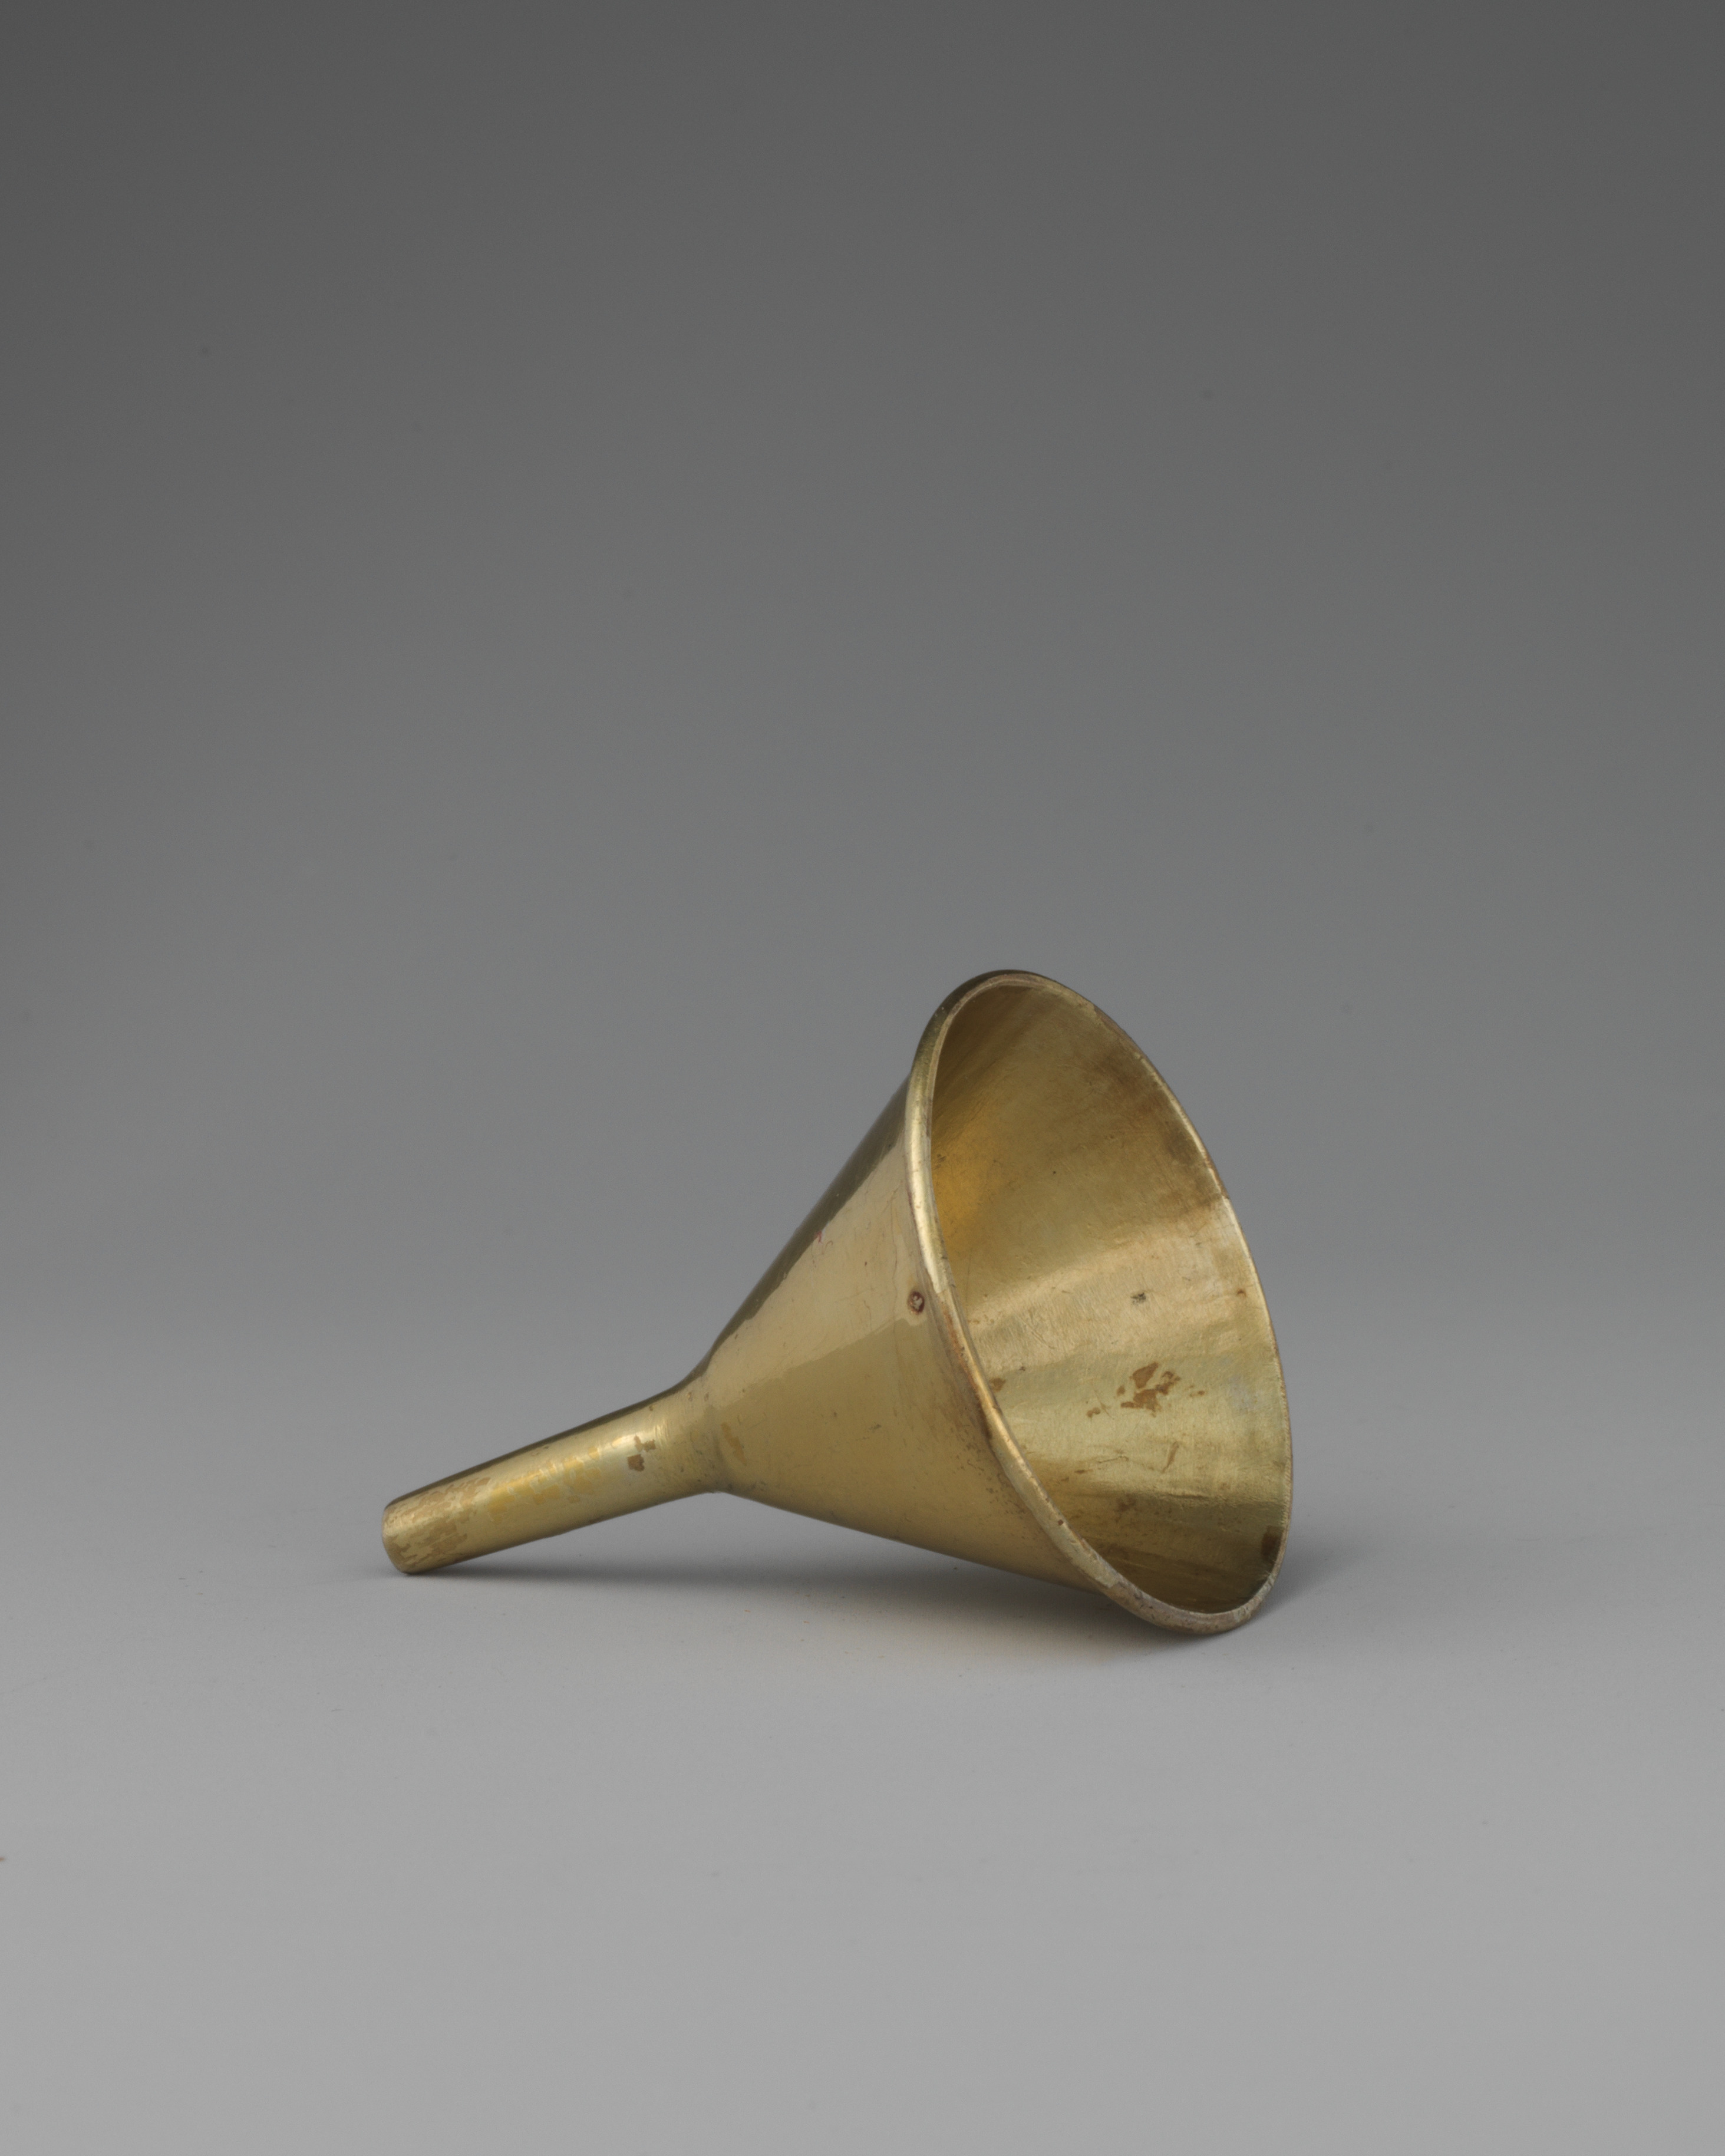
\includegraphics[width=0.5\textwidth]{bilder/01-trichter}
	\caption[Miniaturtrichter]{Miniaturtrichter, 18.~Jahrhundert, Französisch}
	\label{fig:trichter}
\end{figure}


\subsection{Fließbilder}
\label{subsec:fliessbilder}
Können zum Beisiel mit Inkscape erstellt werden. Als Schriftart bietet sich die Dokumentschriftart Libertine oder die Serifenlose Roboto an. Siehe Ordner fonts.

\begin{figure}[h]
	\centering
	\includegraphics[width=0.75\textwidth]{bilder/02-cgam-komplett}
	\caption[Fließbild CGAM-Prozess]{Fließbild CGAM-Prozess}
	\label{fig:cgam-komplett}
\end{figure}

\subsection{Diagramme}
\label{subsec:diagramme}
Diagramme können schnell und einfach mit tikz erstellt werden. Anbei ein Beispiel, siehe \cref{fig:cgam-diagramm}.

\begin{figure}[h]
	\centering
	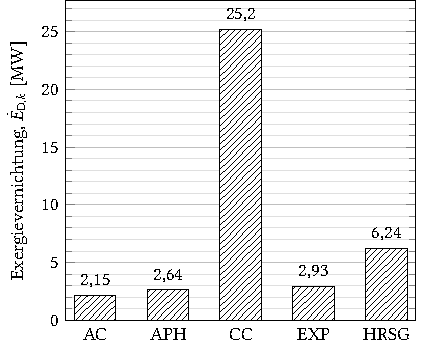
\includegraphics{bilder/03-cgam-diagramm.pdf}
	\caption[Bildunterschrift kurz, für Abbildungsverzeichnis]{Bildunterschrift lang, ggf. mit Verweis auf Quelle}
	\label{fig:cgam-diagramm}
\end{figure}


\clearpage

\section{Tabellen}
\label{sec:tabellen}

Zur Erstellung von Tabellen wird das Paket booktabs genutzt. Auf senkrechte Linien in Tabellen sollte verzichtet werden. Hier ein Beispiel inkl. Tabellenfussnoten. 

%Tabelle mit Schriftgröße 10 (tabular10)
\begin{table}[htbp]
	\centering
	\caption{Parameter der ökonomischen Analyse}
	\label{tab:trr}
	\begin{threeparttable}
		\begin{tabular10}{lllcc}
			\toprule
			Parameter & Symbol & Einheit & Wert \\
			\midrule
			Betriebsdauer, siehe \cite{markewitz2016} & $n$ & a & 40 \\
			Durchschn. nom. Steigerungsrate, universell\tnote{a} & $r_\text{n,uni}$ & \%/a & 1,5 \\
			Fixe Betriebs- und Wartungskosten, s.~\cite{konstantin2013}& $omc_\text{fix}$ & \%/a & 1,5\\
			Variable Betriebs- und Wartungskosten & $omc_\text{var}$ & \euro/MWh\textsubscript{el} & 1,3\tnote{b}\\
			Spezifische Emissionskosten\tnote{a}& $ec$ & \euro/t\ce{CO2} & 20\\
			Emissionsfaktor\tnote{c}& $k_{\ce{CO2}}$ & t\ce{CO2}/MWh\textsubscript{fuel} & 0,34 \\
			\midrule	 
			Äquivalente Jahresvollbenutzungsstunden & $\tau$ & h/a & 4500\\
			Effektiver jährlicher Zinssatz & $i_\text{eff}$ & \%/a & 5\\ 
			Spezifische Brennstoffkosten& $fc$ & \euro/GJ & 1,9\\			
			Durchschn. nom. Steigerungsrate, Brennstoff & $r_\text{n,fuel}$ & \%/a &  2\\
			\bottomrule    
		\end{tabular10}
		\begin{tablenotes}\scriptsize
			\item[a] Annahme
			\item[b] siehe \cite{konstantin2013}
			\item[c] Basierend auf eigenen Berechnungen; Methodik siehe \cite{quick2010}
		\end{tablenotes}
	\end{threeparttable}
\end{table}



\section{Literaturverweise}
\label{sec:literatur}

Mit biblatex und biber lassen sich schnell und einfach Literaturverweise anlegen. Die Optionen für biblatex werden in der Präambel übermittelt. Als Backend wird biber genutzt. Der Eintrag der Quellen erfolgt in einer *.bib Datei. Dazu können auch Literaturverwaltungsprogramme wie jabref (quelloffen) oder Citavi (kostenpflichtig, Lizenz über TU Berlin) genutzt werden.

\subsection{Ein Beispiel mit Zitat}

Die mathematische Beschreibung der stationären Kraftwerkssimulation entspricht sinnvollerweise einem impliziten Gleichungssystem. Statt $y=f(x)$ wird 
\begin{equation}
F\left(x, y\right)=0
\end{equation}
notiert.\footnote{vgl. \cite[S.\,147]{papula2014}} Dies ist unter Umständen sogar zwingend erforderlich, da nach \cite[S.\,260]{westermann2011} "`die Bestimmungsgleichung nur schwer oder gar nicht explizit nach $y=f(x)$ auflösbar [ist]."' Selbst ein einfaches Stoffwertpolynom wie die Darstellung der Entropie bei Referenzdruck nach Knacke et al.\,\cite{knacke1991}, 
\begin{equation}
s^0=\text{S}^++\text{a}\,\ln(T/\text{K})+\text{b}\,y-\frac{\text{c}}{2}\,y^{-2}+\frac{\text{d}}{2}\,y^2\quad\quad\text{mit}\quad y=10^{-3}T/\text{K}
\label{eq:knacke_entropie}
\end{equation}
also lediglich abhängig von der Temperatur, ist nicht analytisch nach $T$ auflösbar.

\subsection{Einfache Verweise auf Literaturquellen}

Zoder et al.~\cite{zoder2018} kommen in ihrem wissenschaftlichen Artikel zu dem Ergebnis, dass der Einsatz exergiebasierter Methoden bei der Analyse von Energieumwandlungsanalgen hilfreich ist.

Andere Autoren legen in ihren teils umfangreichen Publikationen ebenfalls interessante Ergebnisse vor, vgl.~\cite{baehr1979,clausius1850,gasparovic1969,keenan1932,lojewski_urban1989}. Wobei sogenannte \textit{lumped references} vermieden werden sollten. Jede Literaturstelle ist einzeln zu würdigen und es ist zu beschreiben, was aus dieser Quelle übernommen wird bzw, welche Ansätze, Ideen, Erkenntnisse usw. daraus erwähnenswert sind.

Einige Autoren haben lesenswerte Bücher verfasst, darunter Baehr und Kabelac~\cite{baehr2012}, Szargut~\cite{szargut2007} oder Moran et al.~\cite{moran2014}. Nicht zu vergessen Müller~\cite{mueller2001} und die aktuelle Zusammenstellung der IEA~\cite{weo2016}.

Neben Büchern und wissenschaftlichen Artikeln, ist es auch möglich auf Buchbeiträge \cite{lojewski_urban1989}, Tagungsbände \cite{spliethoff2010a}, Beiträge in Tagungsbänden \cite{fraas1974,fraas1975}, Dissertationen \cite{ruegg1945,gaggioli1961}, wissenschaftliche Berichte \cite{gutstein1975,nas_3_10606_1968}, Internetquellen uvm. zu verweisen.

\subsection{Literaturverweis mit Seitenangabe}

Müller notiert dazu die thermische Zustandsgleichung nach van der Waals, siehe~\cite[S.~100]{mueller2001}.












%weitere Kapitel hier einfügen

%\cleardoublepage
%\input{03_neues_kapitel}

%Literatur
\cleardoublepage
\printbibliography[heading=bibintoc]

%Bildnachweise
\cleardoublepage
\chapter*{Bildnachweis}
\addcontentsline{toc}{chapter}{Bildnachweis}

\autoref{fig:trichter}: The Metropolitan Museum of Art,\\
https://www.metmuseum.org/art/collection/search/202901, (CC0 1.0)

%Abkürzungs- und Symbolverzeichnis
\cleardoublepage
\renewcommand{\chaptermark}[1]{\markboth{#1}{}}

\chapter*{Abkürzungs- und Symbolverzeichnis}
\addcontentsline{toc}{chapter}{Abkürzungs- und Symbolverzeichnis}
\label{ch:symbole_abk}
\chaptermark{Abkürzungs- und Symbolverzeichnis}

\noindent 
\textit{Abkürzungen}

\vspace{6pt}

\noindent 
\begin{tabular}{@{}p{2cm}l}
AC&Air Compressor, Luftverdichter\\
APH&Air Preheater, Luftvorwärmer\\
CC&Combustion Chamber, Brennkammer\\
EXP& Expander\\
HRSG&Heat Recovery Steam Generator, Abhitzekessel\\
\end{tabular}

%\clearpage

%\noindent
%\begin{tabular}{@{}p{2cm}l}
%IEA& International Energy Agency\\
%NASA& National Aeronautics \& Space Administration\\
%\end{tabular}

\vspace{18pt}
%\clearpage

\noindent 
\textit{Lateinische Symbole}

\vspace{6pt}

\noindent 
\begin{tabular}{@{}p{2cm}l}
	$c$&Spezifische Kosten je Exergieeinheit, \euro/J\textsubscript{ex}\\
	$\dot C$&Kostenstrom, \euro/h \\
	$CC$&Kapitalgebundene Kosten, \euro \\
	$c\!f$&Capacity Factor, Jährliche Auslastung, --\\	
	$e$&Spezifische Exergie, J/kg\\
	$\bar{e}$&Spezifisch molare Exergie, J/mol\\
	$\dot E$&Exergiestrom, W\\
	$f$&Exergoökonomischer Faktor, --\\
	$fc$&Spezifische Brennstoffkosten, \euro/J\\
	$FC$&Brennstoffkosten, \euro \\
	$h$&Spezifische Enthalpie, J/kg\\
	$\dot H$&Enthalpiestrom, W\\
	$HHV$&Brennwert, J/kg\\
\end{tabular}

\vspace{18pt}
%\clearpage

\noindent 
\textit{Griechische Symbole}

\vspace{6pt}

\noindent 
\begin{tabular}{@{}p{2cm}l}
	$\Delta$&Differenz\\
	$\varepsilon$&Exergetischer Wirkungsgrad, --\\
	$\eta_s$&Isentroper Wirkungsgrad, --\\
	$\kappa$&Isentropenexponenten, --\\
	$\lambda$&Luftzahl, --\\
\end{tabular}

\vspace{18pt}
%\clearpage

\noindent 
\textit{Hoch- und tiefgestelle Indizes}

\vspace{6pt}

\noindent 
\begin{tabular}{@{}p{2cm}l}
	0&Referenzpunkt, Thermodynamische Umgebung\\
	a&Avarage, Mittlere\\
	D&Destruction, Vernichtung\\
	F&Fuel, Brennstoff, Aufwand\\
	net&Netto\\
\end{tabular}


%Abbildungsverzeichnis
\cleardoublepage
\addcontentsline{toc}{chapter}{\listfigurename}
\listoffigures

%Tabellenverzeichnis
\cleardoublepage
\addcontentsline{toc}{chapter}{\listtablename}
\listoftables

%Anhang
\cleardoublepage
\appendix
\part*{Anhang}
\addcontentsline{toc}{chapter}{Anhang}

\chapter{Simulationen -- Fließbilder und Vorgaben}
\label{ch:a_sim}

\section{Fall 1}


\chapter{Kostenrechnung}
\label{ch:a_kosten}


\chapter{Ergebnisse}
\label{ch:a_erg}

\end{document}